\PassOptionsToPackage{utf8}{inputenc}
\documentclass{bioinfo}

\usepackage{natbib}
%\usepackage[
%backend=biber,
%sorting=ynt
%]{biblatex}

\usepackage{makecell}

\usepackage{floatrow}

\usepackage{comment}

\usepackage{siunitx}

% singlelinecheck=false puts subcaptions on the left
\usepackage[singlelinecheck=false]{subcaption}

\usepackage[usenames,dvipsnames]{xcolor}

%\usepackage{amsthm}
% Says package is already imported?
\theoremstyle{definition}
\newtheorem{definition}{Definition}[section]
\newtheorem{theorem}{Theorem}[section]
\newtheorem{corollary}{Corollary}[theorem]
\newtheorem{lemma}[theorem]{Lemma}

\usepackage{algorithm2e}
\SetKwRepeat{Do}{do}{while}%

% we squeeze our figures even more together
\captionsetup{belowskip=-2pt}

\SetAlgoLined
\SetKwProg{MyStruct}{Struct}{ contains}{end}

\newcommand{\vocab}{\textbf}
\newcommand{\red}[1]{{\textcolor{Red}{#1}}}
\newcommand{\FIXME}[1]{\red{[FIXME: #1]}}

\usepackage{orcidlink}
\hypersetup{hidelinks}


\usepackage{graphicx}

\def\labelitemi{--}

\copyrightyear{2023} \pubyear{XXXX}

%\access{Advance Access Publication Date: Day Month Year}
%\appnotes{Genome Analysis}

\begin{document}
\firstpage{1}

%\subtitle{Genome Analysis}

\title[FantasticLamp]{FantasticLamp: quantifying genomic edits with genome variation graphs}
\author[Schutte \textit{et~al}.]{

Casper~Schutte\,$^{\orcidlink{0000-0003-4245-6842}\text{\sfb 1}}$,
Ian~T~Fiddes\,$^{\orcidlink{0000-0002-1580-7443}\text{\sfb 2}}$,
Erik~Garrison\,$^{\orcidlink{0000-0003-3821-631X}\text{\sfb 3}*}$
}

\address{
$^{\text{\sf 1}}$Department of Bioinformatics and Computational Biology, University of Stellenbosch, Stellenbosch, 7600, Western Cape, South Africa \\
$^{\text{\sf 2}}$10x Genomics, Pleasanton, CA \\
$^{\text{\sf 3}}$Department of Genetics, Genomics and Informatics, University of Tennessee Health Science Center, Memphis, 38163, Tennessee, USA \\
}

\corresp{
$^\ast$To whom correspondence should be addressed. \\
% $^\dagger$Contributed equally.\
}

\history{Received on XXXXX; revised on XXXXX; accepted on XXXXX}

\editor{Associate Editor: XXXXXXX}

\abstract{
\textbf{Motivation:}
Accurately calculating the efficacy of genomic edits is crucial to understanding the performance of the editing techniques, in order to optimize methods and improve the success rate of the edits.
Additionally, by understanding the success rate of genomic edits, researchers can identify any potential problems or limitations of the techniques and work to overcome them.
This can help to improve the accuracy and precision of the editing methods, which is essential for many applications, such as creating genetically engineered cells for therapeutic purposes, understanding gene functions, and studying genetic diversity in a population of cells.
Current linear alignment methods for quantifying the success of edits exhibit reference bias and cannot model complex mixed edit states.\\
% Mention current methods and why there is need for better methods.
\textbf{Results:}
We design \textit{FantasticLamp}, an open source genome-graph-based pipeline for calculating the efficacy of genomic edits performed on multiple populations of cells.
It constructs a variation graph from the reference genome and edit template sequences that includes both edited and unedited sequences as paths, and combinations of edits as potential walks through the graph.
It then maps reads from the edited populations onto this graph in order to calculate the coverage of the edited sequences compared to the unedited sequences.
This pipeline aims to provide a quantitative measure of the success of each genomic edit without bias towards the reference or particular single editing constructs.\\
% Reword this paragraph, add detail regarding the process. Mention the successful implementation.
\textbf{Availability:}
\textit{FantasticLamp} is published as free software under the MIT open source license.
Source code and documentation are available at \url{https://github.com/casper-schutte/fantastic-lamp}.
\textbf{Contact:} \href{egarris5@uthsc.edu}{egarris5@uthsc.edu} \\
%\textbf{Supplementary information:} Supplementary data are available at \textit{Bioinformatics} online.
}

\maketitle


\section*{Introduction}
\label{sec:introduction}

In the field of genome engineering, various methods such as CRISPR/Cas9, TALEN, and ZNF-based systems are employed to create genomic edits in cells for the study of gene functions and the creation of new cell lines \citep{gaj2013zfn}.
Identifying and quantifying the success rate of these edits in large-scale data sets can be challenging due to factors such as variations in editing efficiency, unintended off-target effects, and the complexity of accurately distinguishing between successfully edited and unedited sequences \citep{guell2014genome}, \citep{van2020delivery}.
%Identifying and quantifying the success rate of these edits in large-scale data sets can be challenging ... \citep{guell2014genome}, \citep{van2020delivery}.

Traditional approaches that attempt to enumerate all possible edit states as individual target sequences must confront an exponential number of edit combinations.
This can increase complexity and introduce errors \citep{huang2013short}, \citep{mun2021leviosam}.
Moreover, assessing the success rate of genomic edits through a linear alignment method may lead to reference bias, especially when there are multiple nearby edits and mixed edit states.

An alternative to these linear methods is the use of a genome graph approach, which can offer a more comprehensive perspective on sequence relationships, avoiding reference bias, and capturing all allele state mixtures, even in cases of overlapping edits \citep{eggertsson2017graphtyper,Martiniano_2020}.
Genome graphs provide a more accurate and complete view compared to linear alignment methods by allowing reads to be mapped to a graph that represents a population of sequences and the variations between them, rather than a single reference \citep{garrison2018variation,paten2017genome,Eizenga_2020}.

Given the aforementioned advantages of the genome graph approach, we propose \textit{FantasticLamp}, a pipeline tailored for quantifying edit efficacy in experiments involving multiple edits performed on the same population.
This pipeline leverages genome graph-based sequence analysis, offering a more suited solution for this context.

Our method involves mapping genomic edits onto structures representable in variation graphs (Figure \ref{fig:images}A-C).
We subsequently align reads from a population of edited cells to this graph and quantify edit efficiency by comparing the observed edited and unedited allele states (Figure \ref{fig:images}D).
This integrated approach ensures a more accurate quantification of edit efficacy across multiple populations of edited cells.

\section*{Implementation}
\label{sec:implementation}
Here we describe the steps and tools utilized in creating \textit{FantasticLamp}.

Given a reference genome and reads sequenced from multiple edited populations, the pipeline employs a design library file---a table containing the intended edits and reference sequences at the intended edit sites---to construct a genome graph.

The genome graph consists of the reference genome, the intended edit sequences (referred to as ``homology arms'' or ``edit homology arms''), and the reference sequences at the edit sites (termed ``reference homology arms'').
The core structure of the graph is an alignment of homology and reference homology arms onto the reference genome, which we complete using \textit{minimap2} \citep{li2018minimap2}.
The inclusion of the reference homology arms enables the pipeline to calculate the relative coverage, thereby determining the edit efficiency by comparing the coverage of edit homology arms to that of the reference homology arms.

Then, we construct the graph itself.
A variation graph, representing the relationships between the reference genome and both groups of homology arms (reference and edit), is then induced by \textit{seqwish} \citep{garrison2023unbiased}, which combines the input sequences and the alignments into a graph (in GFAv1 format).
After the graph's construction, the nodes are 'chopped' into segments smaller than 256 base pairs to enable efficient indexing and read mapping, and the graph is sorted using \textit{odgi} \citep{guarracino2022odgi}.

The pipeline then maps reads from the edited populations to this graph using \textit{vg} \citep{garrison2018variation}, generating a GAF (Gene Annotation Format) file to represent the alignment.
A Python script parses the alignment file to calculate the coverage of the homology arms relative to the reference homology arms.
We output a coverage table (in TSV format), displaying each intended edit sequence alongside the corresponding homology arm coverage and reference homology arm coverage, thereby quantifying the efficacy of each edit.

\textit{FantasticLamp} thus enables the simultaneous quantification of edit efficacy across multiple edited populations, serving as a valuable tool for both the testing of novel editing methods and the verification of current methods in experiments involving genomic edits.
By aligning reads to a graph instead of employing linear alignment, \textit{FantasticLamp} circumvents reference bias and will allow for precise quantification of genome edit states even in the case of contexts where many simultaneous edits are applied in close proximity.
%in genome engineering and related fields who seek precise quantification of genome edit states. %\\
A flow diagram detailing the steps and files used in the \textit{FantasticLamp} pipeline is presented in Figure \ref{fig:images}D.


%We will discuss the tools used, not in extreme detail but enough to justify and explain their use.
% Mention important functions or at least describe how coverage is calculted, etc. Mention problem of shared reads, plasmid integration, etc.

\section*{Results}
\label{sec:results}
%This pipeline was initially tested and developed using a data set containing sequencing reads %(mention platform) from experiments where multiple edits (insertions, deletions, and substitutions) were performed on a population of \textit{Saccharomyces cerevisiae} (check this) by Inscripta Inc. (ref?). 
%The initial/preliminary results showed/demonstrated/indicated the pipeline's ability to calculate read coverage (and thus efficacy) of the edits performed. 
%Unfortunately, logistical issues prevented continued use of this data set and an artificial test data set was constructed. This artificial data set was comprised of a tiny reference genome, an accompanying design library CSV file containing reference sequences from the genome and edited sequences, and artificial reads mapping to either the reference or the edit at a particular edit locus. 
%The pipeline accurately calculated the edit coverage and thus provided a quantitative measure of edit efficacy.  

The initial development and testing of this pipeline were carried out using a dataset containing sequencing reads from various experiments.
These experiments involved multiple alterations---insertions, deletions, and substitutions---on a population of \textit{Saccharomyces cerevisiae}.
They were performed in distinct batches by Inscripta Inc. \citep{gander2021simultaneous}.

We found that the pipeline captured expected edit states.
However, due to unforeseen logistical constraints, further usage of this dataset was halted.
Consequently, an artificial dataset was constructed for further testing and refinement.

This synthetic dataset encompasses a small reference genome, a related design library CSV, which contain both the reference and edited sequences from the genome, and artificial reads mapping to either the reference or the edit at a specific edit locus. 
\textit{FantasticLamp} accurately calculated the edit coverage from this dataset, providing a quantitative evaluation of the edit's effectiveness.
We provide this as a standard test in our code repository.

For further validation, we created a much larger validation test by taking a full yeast genome (GCF\_000146045.2) and introducing a single edit (ranging from 20 - 25bp) at a specific locus, which we then simulated reads from.
We created 100 of these edited genomes, each with a different edit at a random locus, and simulated 10x coverage, paired-end reads from each genome.
We then ran \textit{FantasticLamp} on two sets of these simulated reads; one set with a base error rate of 0.5\%, and one with a base error rate of 1\%.
In both of these validation tests, \textit{FantasticLamp} was able to identify the correct edit state for 97 out of 100 edits.
The scripts used to generate these genomes and reads (as well as to perform the actual validation tests) are available in the code repository.

%\begin{figure}
%	\centering
%	\fbox{\includegraphics[width=\columnwidth]{flow.pdf}}
%	\caption{Test Caption for Insertion}
%	\label{fig:insert}
%\end{figure}

%\begin{figure}
%	\fbox{\includegraphics{deletion.pdf}}
%	\caption{Test Caption for Deletion}
%	\label{fig:deletion}
%\end{figure}
%
%\begin{figure}
%	\fbox{\includegraphics{substitution.pdf}}
%	\caption{Test Caption for Substitution}
%	\label{fig:substitution}
%\end{figure}


\begin{figure}[htbp]
	\centering
	\begin{minipage}[b]{0.35\columnwidth}
		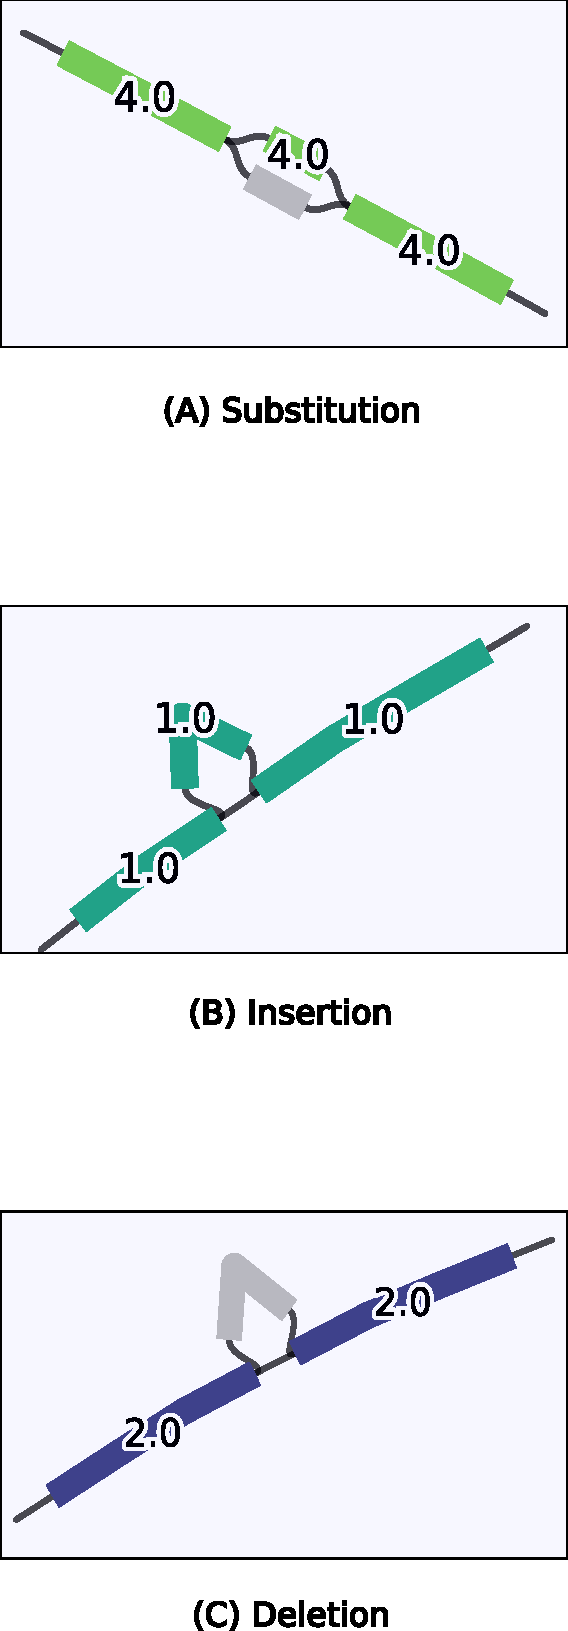
\includegraphics[width=\textwidth]{panels.pdf}
		%\caption{Test caption for panel figure}
		\label{fig:panel}
	\end{minipage}
	\hfill
	\begin{minipage}[b]{0.64\columnwidth}
		\centering
		\fbox{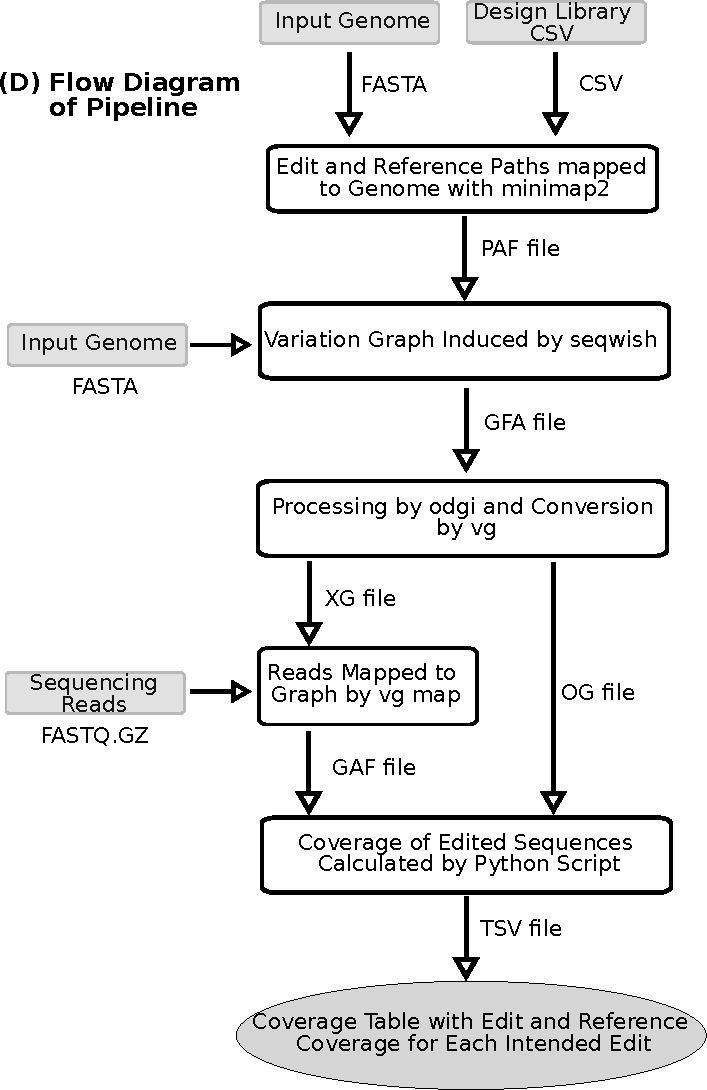
\includegraphics[width=\textwidth]{flow_test.pdf}}
		%\caption{Test caption for flow diagram}
		\label{fig:flow}
	\end{minipage}
	\caption{(A) Graph representation of a substitution. Edit path shown in green. (B) Graph representation of an insertion. Edit path shown in light blue. (C) Graph representation of a deletion. Edit path shown in dark blue. (D) Diagram depicting the steps, software tools, and file formats use in the \textit{FantasticLamp} pipeline.}
	\label{fig:images}
\end{figure}

\section*{Discussion}
\label{sec:discussion}
\textit{FantasticLamp} demonstrates using a variation graph to quantify complex genome edits.
We consider this work as an example of how to apply unbiased edit quantification to editing experiments.
However, much work is left to be done to use these approaches at scale.

As an emerging field, commodity high-throughput genome editing is still uncommon, and accepted standards for experimental design are lacking.
Therefore, the inputs and outputs of our implementation are necessarily customized.

This pipeline provides a starting point to avoid bias when quantifying edits that can be built upon as editing technologies advance.
In this paper, we demonstrate basic functionality of \textit{FantasticLamp} on artificial and singleplex data. 
Using a large validation test, we confirmed the robustness and accuracy of the approaches outlined in this paper.
Moreover, the potential of \textit{FantasticLamp} extends beyond singleplex data, as it could be further developed to analyze multiplexed pooled data.
Other potential improvements include handling more complex structural variants, incorporating multiplexed data, estimating off-target effects, and optimizing runtime for large genomes.
In summary, \textit{FantasticLamp} provides a basic demonstration of the principle of using a variation graph as a reference system to avoid bias when accurately quantifying genomic edits.

\begin{comment}
\section*{Discussion}
\label{sec:discussion}
As novel genome editing processes are developed in the near future, we posit that the need for software tools that can capture the complexity of the edits and the relationship between them will increase.
We show a basic approach for quantifying complex genome editing results, which are difficult to reliably and simply evaluate using a single reference genome that may lead to biased estimates of edit states.
The design library CSV file used in the creation of this pipeline was unique to a specific set of editing experiments performed at Inscripta Inc.
However, the basic format is generic to other editing experiments that users may carry out in the future, with only minimal changes to the script to adjust for difference in formatting of the design library file.
Future users will have to edit the bash script `find\_coverage.sh' such that the correct columns containing the edit- and reference homology arms are extracted.
While the pipeline was tested on artificial data and singleplex sequencing data, it is possible to perform analysis using pooled sequencing data, but data availability has limited our ability to thoroughly test this.
In summary, \textit{FantasticLamp} provides a basic demonstration of the principle of using a variation graph as a reference system to avoid bias when quantifying genomic edits, and stands as a prototype for future work in this space.
\end{comment}

\section*{Acknowledgements}
We are grateful to Inscripta Inc for providing the data from editing experiments that was used to create and test this pipeline. We thank Deanna Church for supporting our collaboration.

\section*{Funding}
The authors gratefully acknowledge support from National Institutes of Health/NIDA U01DA047638 (E.G.), National Institutes of Health/NIGMS R01GM123489 (E.G.), and NSF PPoSS Award \#2118709 (E.G.), and the Center for Integrative and Translational Genomics (E.G. and C.S.).

% Don't think this applies? Check with Erik
\section*{Data availability}
The scripts that comprise the \textit{FantasticLamp} pipeline, as well as the code and links to data resources used to build this manuscript and its figures, can be found in the paper's public repository: \url{https://github.com/casper-schutte/fantastic-lamp}.

\section*{Conflict of interest}
The authors declare that they have no conflicts of interest.

\bibliographystyle{natbib}
\bibliography{document}

\end{document}
